\documentclass[11pt]{article}

%
% Template for GFD reports.
%
% Updated 12/2000.  Address all complaints to Jean-Luc Thiffeault,
% jeanluc@mailaps.org
%
% Updated for 2004 (SDM).
%

%
% Packages (do not delete any!)
%

% This package handles embedded postscript figures.
\usepackage{graphicx}
% The amsmath and amssymb packages provide some extra commands/fonts.
\usepackage{amsmath,amssymb}

% The margins:
\usepackage[body={6in,8.5in}]{geometry}

% LEAVE THESE NEXT TWO LINES IN (used in final version for page numbering).
%\usepackage{lastpage,xr}
%\externaldocument[pr-]{../<previousrep>/rep_<previousrep>}

% The citation format to use.
\bibliographystyle{pfa}

% Add your own packages here, if necessary.

%
% Definitions
%
%
% Symbols file GFD2002
%

% Partial derivative
\def\pd{\partial}
% Real numbers
\def\reals{{\mathbb R}}
% 1st partial derivative
\newcommand {\pdd}[2]{\frac{\partial #1}{\partial #2}}
% 2nd partial derivative
\newcommand {\pdTwo}[2]{\frac{\partial^{2} #1}{\partial #2^{2}}}
% reference style
%\newcommand {\nref}[1]{~(\ref{#1})}
\newcommand {\nref}[1]{~\ref{#1}}
% unit vector notation
\newcommand {\unitv}[1]{\mathbf{\hat{#1}}}
% the subscript for the horizontal component
\newcommand {\horiz}{_{_{H}}}
% the symbol for the velocity
\newcommand {\vel}{\mathbf{u}}
% the symbol for the horizontal velocity
\newcommand {\uh}{\vel\horiz}
% the symbol for the vertical unit vector
\newcommand {\khat}{\unitv{k}}
% the symbol for the unit vector in th y direction
\newcommand {\jhat}{\unitv{j}}
% the symbol for the unit vector in the direction \hnabla h
\newcommand {\nhat}{\unitv{n}}
% the symbol for the horizontal nabla
\newcommand {\hnabla}{\nabla\!\horiz}
% the symbol for the horizontal laplacian
\newcommand {\hlap}{\hnabla^{\,2}}
% the subscript denoting top
\newcommand {\up}{_{_{T}}}
% the subscript denoting bottom
\newcommand {\down}{_{_{B}}}
% degree symbol
\newcommand {\degree} {^{\circ}}
% Cross product
\def\cross{\times}


% Define your own commands here, or input them externally (say, mysymbols.tex).
%\input{mysymbols}
\newcommand{\grad}{\nabla}

%
% Title
%
\title{Tidal Power}
\author{Chris Garrett}

\begin{document}

\maketitle

% LEAVE THESE NEXT TWO LINES IN (used in final version for page numbering).
% They must go right after the \maketitle command.
%\setcounter{page}{\pageref{pr-LastPage}}
%\addtocounter{page}{1}

%%%%%%%%%%%%%%%%%%%%%%%%%%%%%%%%%%%%%%%%%%%%%%%%%%%%%%%%%%%%%%%%%%%%%%%%%%%%%%%

\section{Introduction}
\label{Intro}

The maintenance and extension of our current standard of living will always require the utilization of new energy sources. The current demand for oil cannot be sustained forever, and as scientists we should always try to keep such needs in mind, and oceanographers may be able to help alleviate society's demand for natural resources in some way.

Some suggestions include the oceans in a supportive manner. It may be possible, for example, to use tidal currents to cool nuclear plants, and a detailed knowledge of deep ocean flow structure could allow for the safe dispersion of nuclear waste. But we could also look to the ocean as a renewable energy resource. A significant amount of oceanic energy is transported to the coasts by surface waves, but rough estimates suggest that nearly $100 \ \textrm{km}$ of coastline would need to be developed to absorb a significant amount of energy. Strong offshore winds could also be used, and wind turbines have had some limited success in this area.

But another option is to take advantage of the tides. Although winds and solar radiation are the dominant energy inputs of the ocean, they tend to produce flows that are generally turbulent and it is usually difficult to extract large amounts of energy from them. The tides, however, provide a moderately strong and coherent forcing that we may be able to effectively siphon in some way. In this section, we first consider some of the various ways to extract potential energy from the rising tides, using barrages across estuaries or tidal locks in shoreline basins. We then provide a more detailed analysis of tidal fences, where turbines are placed in a channel with strong tidal currents, and we consider whether such a system could be a reasonable power source.

%%%%%%%%%%%%%%%%%%%%%%%%%%%%%%%%%%%%%%%%%%%%%%%%%%%%%%%%%%%%%%%%%%%%%%%%%%%%%%%

\section{Barrages and Tidal Locks}
\label{BarragesLocks}

The traditional approach to tidal power is with barrages, where a dam is set up to trap water at high tide and then release it through turbines at low tide, after the changing tidal forces have increased the potential energy of the trapped water. So a barrage plant will maximize its energy in a location with a large surface area and maximal tidal amplitude. The following table shows some of the most tidally active regions of the world:
\begin{center}
\begin{tabular}{|c|c|c|}
\hline
& Mean Tidal Amplitude (m) & Basin Area ($\textrm{km}^2$) \\
\hline
La Rance, France & 4 & 17 \\
\hline
Bay of Fundy, Canada & 5.5 & 240 \\
\hline
Annapolis Royal, Nova Scotia & 3.2 & 6 \\
\hline
Severn Estuary, Great Britain & 4 & 420 \\
\hline
Garolim Bay, South Korea & 2.5 & 85 \\
\hline
\end{tabular}
\end{center}

The only major barrage plant is located at La Rance, Brittany, on the northern coast of France, which began operation in 1967. It has an output of 240 MW making it a significant energy source, given that typical coal and nuclear plants have an output of about 1000 MW. A disadvantage of this method is that the power source is clearly an intermittent one, which is why there is a compromise between releasing the energy at the lowest tide and at the period of greatest demand. La Rance was supposed to be the first of many tidal plants across France but their nuclear program was greatly expanded around this time, and so La~Rance remains the only major tidal power plant in the world today. Although it has had an impact on the local ecology, the change has not been severe and it has been argued that the ecology was not particularly unique to begin with.

The only other commercially viable barrage plant is the Annapolis Royal station in Nova Scotia, which was activated in 1982 and has an output of about 20 MW. It was designed as an experimental station that would lead to an array of tidal power stations across the Bay of Fundy, which is not only very large, but it also possesses the largest tides in the world. Such a network may be able produce an energy output as large as 5000 MW, but the environmental consequences could be severe; the more dire of predictions suggest that it could lead to a 5\% drop in the Bay of Fundy tidal levels and a 10\% \emph{rise} in New England's levels. In any case, a better understanding of the effects of such a network would be needed before such an ambitious project can be attempted.

Other barrage plants exist, such as in Russia and China, but none have an output greater than about 500 kW. But the most dramatic of all proposed tidal plants is for a barrage across the Severn Estuary, between Wales and England. There is the possibility that over 8000 MW of power could be extracted, which could supply 12\% of the current UK energy demand. Evaluations were conducted from 1974 to 1987, but the project was eventually shelved because of economic and environmental concerns.

An alternative to barrages is to use the tidal flow through coastal basins with what is sometimes called a tidal lock. The principle is similar to the barrage in that we trap water at high tide and release it through turbines at low tide, but the major difference is that we are able to rectify the current by, say, directing it to enter through the eastern half of the inlet and having it leave through the western half. By using a directed tidal flow along a coastline, we gain the benefit of a barrage without the ecological damage caused by the dams or the intrusion upon coastal shipping. Korea, which currently imports most of its energy, has very large tides and many basins along its shore. Since they have already been using dams in an aggressive land reclamation project for years, they are attempting to couple this with the development of these kind of tidal plants. However, recent attempts have not been able to extract a significant amount of power.

%%%%%%%%%%%%%%%%%%%%%%%%%%%%%%%%%%%%%%%%%%%%%%%%%%%%%%%%%%%%%%%%%%%%%%%%%%%%%%%

\section{Tidal Fences}
\label{TidalFences}

Instead of directly using the variable potential energy of the oceans, it may be possible to utilize the strong tidal currents that are generated through narrow channels in certain parts of the world. We will attempt to quantify the actual amount of power that could be extracted from such a plant. This analysis has been done previously by Garrett and Cummins.\cite{Garrett2004}

We consider flow through a channel of variable cross-section (Fig. \ref{ChannelFigure}).  The current speed $u(x,t)$ is  assumed to be function of time $t$ as well as $x$, but independent of the cross-channel position.
\begin{figure}
\centerline{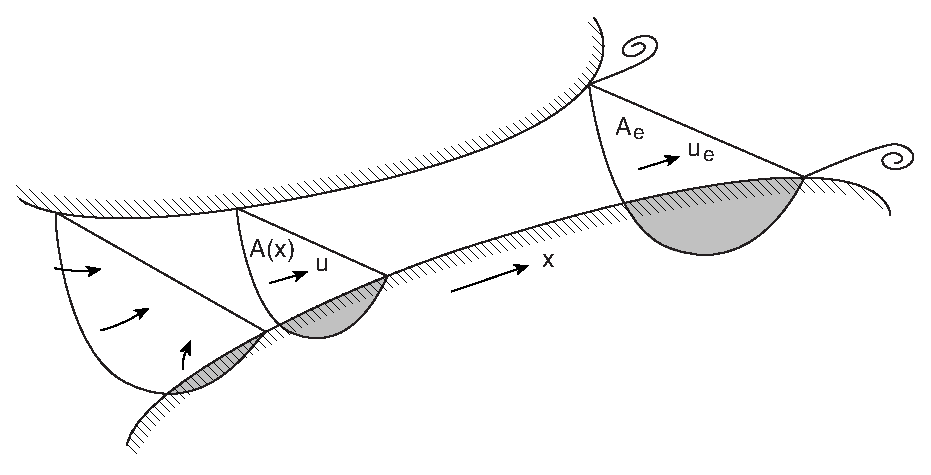
\includegraphics[width=250pt]{Channel_i5b.eps}}
\caption{\footnotesize A channel connects two basins with different tidal elevations. At any instant, the current through the channel has speed $u$, a function of the local cross-sectional area $A(x)$, where $x$ is the along-strait coordinate. At the channel entrance,  the current enters from all directions, but at the exit it may separate as a jet with speed $u_e$, surrounded by comparatively stagnant water with elevation the same as that in the downstream basin.}
\label{ChannelFigure}
\end{figure}
The dynamical equation governing the flow is
\begin{equation}
\pdd{u}{t} + u\pdd{u}{x} + g\pdd{\zeta}{x} = - F
\end{equation}
where the slope of the surface elevation $\zeta$ provides the pressure gradient to drive the flow and $F$ represents an opposing force associated with natural friction and possibly the presence of turbines (in a uniform ``fence'' across the flow, a more efficient scheme than isolated turbines$^6$).

If the channel is short compared with the wavelength of the tide (generally hundreds of kilometers even in shallow water), volume conservation implies that the flux along the channel $Au=Q(t)$, independent of $x$. (We neglect small changes in $A$ associated with the rise and fall of the tide.) Using this in (1) and integrating  along the channel implies
\begin{equation}
c\frac{dQ}{dt} - g \zeta_0 = -\int_0^L F \, dx - \frac{1}{2} u_e |u_e|
\end{equation}
where $c = \int_0^L A^{-1} \, dx$ and $\zeta_0(t)$ is the sea level difference between the two basins, assuming that this difference is unaffected by the flow through the channel. We note that, if $A$ increases rapidly at the ends of the channel, then the geometrical factor $c$ is insensitive to their locations at $x = 0, L$. We allow for flow separation at the channel exit, with $u_e$ denoting the current speed there.

We start by assuming that the natural frictional term and the head loss associated with separation at the exit are small, so that the natural regime has a balance between the sea level difference and acceleration. For $\zeta_0 = a\cos\omega t$, a sinusoidal tide with amplitude $a$ and frequency $\omega$, $Q = Q_0 \sin\omega t$ where $Q_0 = ga(\omega c)^{-1}$. The power generated at the turbines is the integral along the channel of the product of water density $\rho$, current $u$, cross-section $A$, and the local frictional force $F$ representing the turbines. Thus the average power extracted from the flow by the turbines is
\begin{equation}
P = \overline {\int_0^L \rho F Q \, dx} = \rho \overline {Q \int_0^L F \, dx},
\end{equation}
with the overbar indicating the average over a tidal cycle. This would need to be multiplied by a turbine efficiency factor to give the electrical power produced.

We first assume that the drag associated with the turbines is linearly proportional to the current. Then we may write $\int_0^L F \, dx = \lambda Q$ and $P = \lambda \rho \overline {Q^2}$, where $\lambda$ is related to the number of turbines and their location along the channel.  The governing equation
\begin{equation}
c\frac{dQ}{dt} - g a \cos \omega t = -\lambda Q
\end{equation}
is easily solved to give
\begin{equation}
Q = \textrm{Re}\left[ \left(\frac{ga}{\lambda - ic\omega}\right)
e^{-i\omega t}\right],
\qquad P = \frac{{\frac{1}{2}}\rho\lambda g^2a^2}{\lambda^2 + c^2\omega^2}.
\end{equation}

As expected, $P$ at first increases with $\lambda$ (more power is generated as more turbines are added), but then decreases as too many turbines choke the flow. The maximum power, obtained when $\lambda = c\omega$, is
\begin{equation}
P_\textrm{max} = \frac{1}{4} \rho g^2 a^2 (c \omega)^{-1} = \frac{1}{4} \rho c\omega Q_0^2.
\end{equation}
The flow through the channel is then reduced to $2^{-{1/2}}$, or 71\%, of its original value. We also note that this maximum power is independent of the location of the turbines along the channel (with the fewest being needed if they are deployed at the smallest cross-section). This result is independent of the representation of the turbine drag.

A more realistic representation of the turbine drag would be quadratic in the current speed. We have considered an arbitrary exponent, by non-dimensionalizing with $t = \omega^{-1}t'$, $Q=Q_0Q'$, numerically solving
\begin{equation}
\frac{dQ'}{dt'} -\cos t' = -\lambda' |Q'|^{n-1}Q'
\end{equation}
and evaluating $P/ P_\textrm{max} = 4\lambda'\overline{|Q'|^{n-1}Q'^2}$ as a function of $\lambda'$ for different values of $n$ (Fig. 2).
\begin{figure}
\centerline{\includegraphics[width=250pt]{P(n).eps}}
\caption{\footnotesize The scaled maximum power as a function of a parameter $\lambda'$ representing the number of turbines in the channel, for various  values of $n$, where the turbine drag is assumed proportional to the $n$th power of the current speed.}
\label{Fig2}
\end{figure}
The maximum power  for $n=2$ (quadratic drag) is very close to the value $P_\textrm{max}$ derived for $n=1$, and it does not seem that any other drag law could lead to more power.

We thus take $P_\textrm{max}$ as a reasonable estimate of the maximum power available in the case of negligible background friction and exit separation effect. We may evaluate it in terms of conditions at the constriction with smallest cross-sectional area, $A_{\rm min}$, where the amplitude of the undisturbed tidal current is $u_\textrm{max}$, if we write $c = \int_0^L A^{-1} \, dx = L_\textrm{eff}/A_\textrm{min}$, noting that this effective length $L_{\rm eff}$ is likely to be considerably less than the total channel length $L$. Then
\begin{equation}
P_\textrm{max} = \frac{1}{4} \rho \omega L_\textrm{eff}A_\textrm{min}u_\textrm{max}^2.
\end{equation}
This may be compared with the reference value
\begin{equation}
P_0 = \frac{1}{2}\rho A_\textrm{min}\overline{|u_\textrm{max}\cos\omega t|^3}
= \frac{2}{3\pi} \rho A_\textrm{min}u_{\rm max}^3
\end{equation}
which gives the average undisturbed energy flux through the channel and is usually used as an estimate. The ratio is
\begin{equation}
\frac{P_\textrm{max}}{P_0} = \frac{3\pi}{8} \frac{\omega L_\textrm{eff}}{u_\textrm{max}}
\end{equation}
and can either be less than 1 (short channel, strong currents) or greater than 1 (vice versa). For example, with $\omega = 1.4\times 10^{-4}\,$s$^{-1}$, as for the semidiurnal tide, $L_\textrm{eff} = 5$\,km, and $u_{\rm max} = 3$\,m\,s$^{-1}$, then ${P_\textrm{max}/ P_0} = 0.3$, so $P_0$ would overestimate the resource. With these values and $A_\textrm{min} = 5\times 10^5$\,m$^2$ (as for a width of 5\,km and a depth of 100\,m),  then $P_\textrm{max}=800$\,MW.

The calculations so far have neglected background friction and separation effects. If these can be lumped together in a single term, as for quadratic friction in the channel, and represented by a value $\lambda_0$ in (7), we may still solve (7) but the power from the turbines is now $(\lambda' - \lambda _0)/\lambda'$ times the value calculated with $\lambda_0 = 0$. Here we examine the situations in which the acceleration is much less important than friction in the channel (as for a shallow channel) or the separation effect (as for a short channel). The momentum equation is then
\begin{equation}
-g\zeta_0 = -\int_0^LF_\textrm{turb}\,dx - \alpha Q|Q|,
\end{equation}
giving a balance at any instant between the surface slope, the drag associated $\int_0^LF_{\rm turb}\,dx$ with the turbines, and the internal friction and separation, where
\begin{equation}
\alpha = \int_0^LC_d(hA^2)^{-1}\,dx + \frac{1}{2} A_e^{-2}.
\end{equation}
Here $C_d$ is the drag coefficient, $h$ the water depth, and $A_e$ the cross-sectional area at the exit.

In the absence of turbines, the volume flux is $|Q_0| = (g|\zeta_0|/\alpha)^{1/2}$. With turbines, the instantaneous power is $\rho Q(g\zeta_0 - \alpha Q|Q|)$. This has a maximum of
\begin{equation}
P_\textrm{max} = (2/3^{3/2})\rho \overline {Q_0g\zeta_0} = 0.38  \times 
\rho \overline {Q_0g\zeta_0}
\end{equation}
where we have also averaged over a cycle. The flow at any instant is $3^{-1/2} = 0.58$ of what it was in the absence of the turbines, and 2/3 of the head loss along the channel is now associated with their operation.

If the friction within the channel is much less important than the separation effect, (13) may be written
\begin{equation}
P_\textrm{max} = 0.38 \times \frac{1}{2}\rho A_e\overline {|u_{e0}|^3}
\end{equation}
where $u_{e0}= (2g\zeta_0)^{1/2}$ is the exit speed at any instant in the natural regime. This formula is similar to (9), but we note the reduction factor of 0.38 and, particularly, the fact that it must be evaluated at the exit, likely giving a considerably lower value than would be obtained at the most constricted part of the channel. The turbines could still be deployed there, however.

In the preceding analysis we have assumed that the current is independent of the cross-sectional position. If there is shear vertically and across the channel, we may deal with the average speed in the acceleration term, but there will be minor changes in other parts of the theory. We have also ignored the back effect of changes in the channel flow on the forcing tides. This is likely to be small if the basins are large and deep, but there may be a positive feedback which will increase the head as turbines are introduced. This will slightly increase the available power.

Further consideration for particular sites will require more detailed analysis, but (8), (13) or (14), whichever is appropriate, will still give a good preliminary estimate of the power potential of a number of suggested sites around the world. We emphasize that the commonly used estimate, based on the energy flux in the natural state through the smallest cross-section, is incorrect and likely to be an overestimate.  In general, significant power potential depends not only on the  obvious factors of strong currents and large cross-section, but also on either the channel being long, or the currents at the exit separation, rather than just the constriction, being large.

\noindent \emph{Notes by Viswewaran Nageswaran and Marshall Ward.}

%%%%%%%%%%%%%%%%%%%%%%%%%%%%%%%%%%%%%%%%%%%%%%%%%%%%%%%%%%%%%%%%%%%%%%%%%%%%%%%

% You can add your own bibliography file (say, mybib.bib) here:
\bibliography{gfd2004,lecture10}
%\bibliography{gfd2004}

\end{document}
